\documentclass[../thesis.tex]{subfiles}
\begin{document}
\chapter{Background}\label{cap:background}
This chapter provides an explanation of the main technologies involved in the thesis. It illustrates the chosen serverless solutions, the NodeJS library for headless browser automation and the platform to perform data ingestion and searching. A note should be made on containerization and orchestration processes performed with \gls{docker} and \gls{k8s}, respectively. Due to the popularity of these two tools, it has been decided to not describe them in this chapter and to consider them as already known.

\autoref{sec:aws_lambda} describes the serverless computing platform provided by \acrshort{AWS}, \autoref{sec:knative} analyzes the open-source serverless application layer incubated and supported by \acrshort{CNCF}. \autoref{sec:puppeteer} explains how the browser automation happens and what can be achieved using the library. Finally, \autoref{sec:elasticsearch} introduces some history of the tool chosen to perform data ingestion and searching, from its origins to its more technical aspects such as an installation example.

\section{AWS Lambda}\label{sec:aws_lambda}
\acrshort{AWS} Lambda is a serverless compute service provided by \acrlong{AWS} which allows code to be executed without provisioning or managing servers. All of the administration of the compute resources, including server and operating system maintenance, capacity provisioning, automatic scaling, and logging is performed on a high-availability compute infrastructure. As a serverless service, Lambda only runs functions when an event occurs with a pay-as-you-go billing model \cite{site:aws_lambda_doc}. It integrates seamlessly with other \acrshort{AWS} services to invoke functions or perform other actions, exploiting previously configured triggers or event source mapping. Some examples of well-connected services are API Gateway, \acrshort{S3}, \acrshort{SQS}, \acrshort{SNS}, \gls{dynamo_db}, etc. 

Lambda uses a secure and isolated execution environment that manages the resources required to execute the function, the latter also provides lifecycle support for the function's runtime and any external extensions associated with it. \autoref{fig:aws_lambda_architecture} and \ref{fig:aws_lambda_lifecycle} show the components of this isolated environment, and illustrate the runtime phases of the function.

\begin{figure}[H]
    \centering
    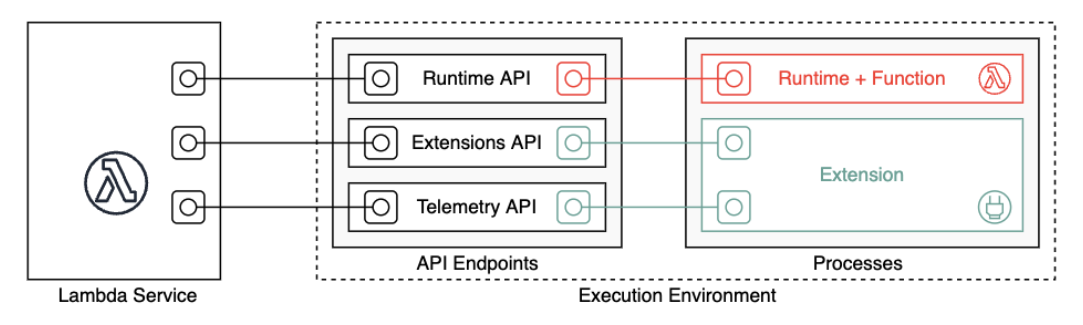
\includegraphics[width=1\textwidth]{background/aws_lambda_architecture.png}
    \caption[Lambda execution environment]{The function's runtime communicates with Lambda using the Runtime \acrshort{API}. Extensions communicate with Lambda using the Extensions \acrshort{API} and they can also receive log messages and other telemetry from the function by using the Telemetry \acrshort{API}. Picture from \href{https://docs.aws.amazon.com/lambda/latest/dg/lambda-runtime-environment.html}{AWS Lambda}.}
    \label{fig:aws_lambda_architecture}
\end{figure}

\begin{figure}[H]
    \centering
    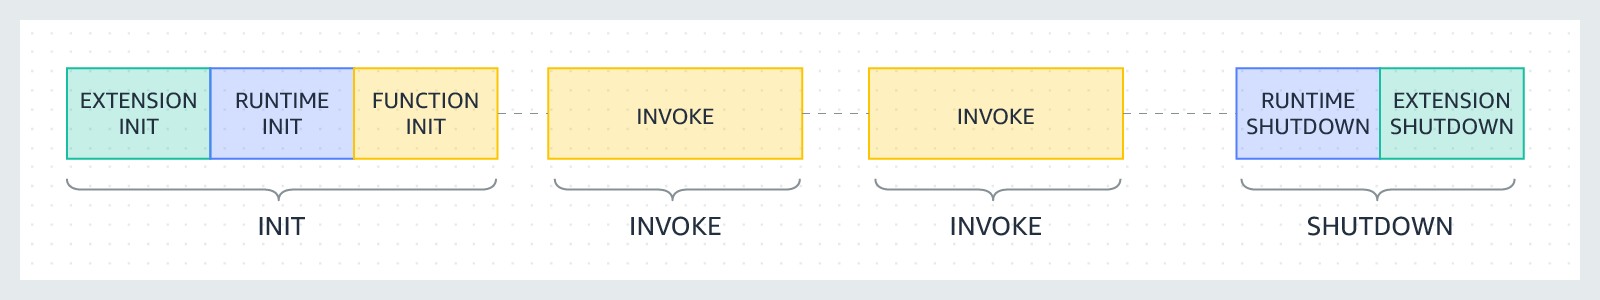
\includegraphics[width=1\textwidth]{background/aws_lambda_lifecycle.png}
    \caption[Lambda execution environment lifecycle]{The Lambda execution environment lifecycle is composed of three phases: Init, Invoke and Shutdown. During the Init phase, the environment is prepared for the invocation of the Lambda function (download code, init extensions and runtime environments, load code). The Invoke phase occurs when the function is invoked, and the Shutdown phase freezes the execution environment when the runtime and extensions have completed their tasks. Picture from \href{https://docs.aws.amazon.com/lambda/latest/dg/lambda-runtime-environment.html}{AWS Lambda}.}
    \label{fig:aws_lambda_lifecycle}
\end{figure}

The code downloaded and executed inside a function is composed of scripts or compiled programs with their dependencies. There are two available options that Lambda supports to deploy these files:

\begin{itemize}
    \item \gls{container} images, includes the base operating system, the runtime, Lambda extensions, application code and its dependencies;
    \item .zip archives, include an application code and its dependencies; it is created by default when a Lambda console or a toolkit is used.
\end{itemize}

In our case, the \gls{container} image was chosen as the deployment package because the dependencies exceeded the size allowed by the zip archive. In addition, using the \gls{container} image enables a static vulnerability analysis to be performed on the code.

\section{Knative}\label{sec:knative}
Knative is a layer over \gls{k8s} that solves common problems of deploying, upgrading and observing software, connecting disparate systems together, routing traffic, and scaling automatically \cite{site:knative}.

Its implementation was originally started by Google but is maintained by the community, which includes people from companies like Red Hat, Google, IBM and VMware. As mentioned, this project was accepted by the \acrshort{CNCF} at the incubation maturity level on 2 March 2022 and recently, a graduation proposal was made by \citeauthor{site:knative_graduation} \cite{site:knative_graduation}.

In short, it can be defined as a platform-agnostic solution for running serverless deployments or, in more detail with the following quote:
\say{Knative is a developer-focused serverless application layer which is a great complement to the existing \gls{k8s} application constructs. Knative consists of three components: an HTTP-triggered autoscaling container runtime called Knative Serving, a CloudEvents-over-HTTP asynchronous routing layer called Knative Eventing, and a developer-focused function framework which leverages the Serving and Eventing components, called Knative Functions} \cite{site:knative_cncf_project}.

There are several methods to install Knative in a cluster, and each was adapted to specific use cases and implementation scenarios.

\begin{itemize}
    \item quickstart plugin: an easy-to-use plugin in which you can specify Minikube or Kind\footnote{Minikube and Kind are two tools that allow the creation of \gls{k8s} clusters locally, so you can have a local development environment. See \href{https://kubernetes.io/docs/tasks/tools/}{https://kubernetes.io/docs/tasks/tools/} for more details.} to create a local \gls{k8s} cluster, which includes the installation of a simplified version of Knative, only for development purposes;
    \item \acrshort{YAML}-based installation: a more comprehensive option for deploying Knative in production environments, which involves applying \acrshort{YAML} files using 
\texttt{kubectl} \acrshort{CLI} to establish Knative's main components and extensions;
    \item operator: an automated and managed installation process for the Knative components in a production environment.
\end{itemize}

In our case, the \texttt{quickstart} plugin was used during the development, and the \acrshort{YAML}-based installation was chosen in the production environment.

At this point, it is possible to interact with the cluster and Knative components in a classical way using \texttt{kubectl}. Another method is to use \texttt{kn}\cite{site:knative_cli_tools} \acrshort{CLI}, which provides a simple and fast interface for creating Knative resources and simplifies completing otherwise complex procedures such as autoscaling and traffic splitting.

\subsection{Serving}
Knative Serving defines a set of objects, such as \gls{k8s} \acrlong{CRD}s, to control the behaviour of serverless workloads on the cluster. \autoref{fig:knative_serving_components} shows how these resources interact with each other, providing many simplifications for the user, when managing deployment or maintenance. A description of each is given below:

\begin{figure}[H]
    \centering
    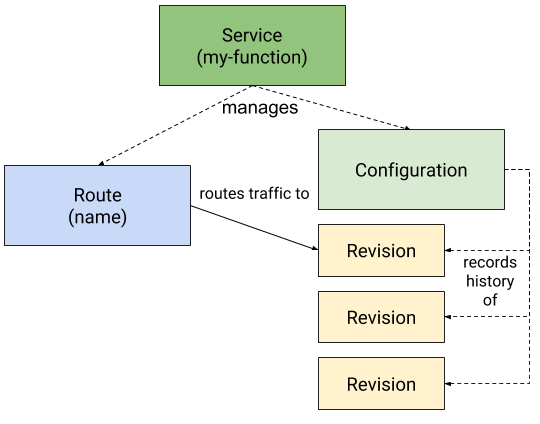
\includegraphics[width=.7\textwidth]{background/knative_serving_components.png}
    \caption[Primary resources in the Knative Serving \acrshort{API}]{Diagram showing the primary resources of Knative Serving \acrshort{API} and how they interact with each other. Picture from \href{https://knative.dev/docs/serving/architecture/\#diagram}{Knative}.}
    \label{fig:knative_serving_components}
\end{figure}

\texttt{Service} Automatically manages the entire workload lifecycle and checks if all the necessary resources (route, configuration, revision) are up and running without problems. It is possible to define to which revision the traffic should be directed.

\texttt{Route} Maps a network endpoint to one or more revisions, making it possible to split traffic and create named routes.

\texttt{Configuration} Maintains the desired state of the deployment and provides a clean separation between code and configuration, following the Twelve-Factor App\footnote{The Twelve-Factor App methodology is a set of best practices that can help in building modern, cloud-native applications that are scalable, reliable, and maintainable. See \href{https://12factor.net/}{https://12factor.net/} for more details.} methodology. When a configuration is changed, a new revision is automatically created.

\texttt{Revision} Represents an immutable snapshot of the application code and configuration. It can be scaled up and down automatically according to incoming traffic and enables progressive roll-out and roll-back of application changes. If idle for a certain period of time, it is automatically cleaned up by garbage collection, thus freeing cluster resources.

The logical components involved in creating a Knative Service were presented and illustrated. \autoref{fig:knative_serving_architecture} is intended to describe all components of the architecture that manage the serverless workflow.

\begin{figure}[H]
    \centering
    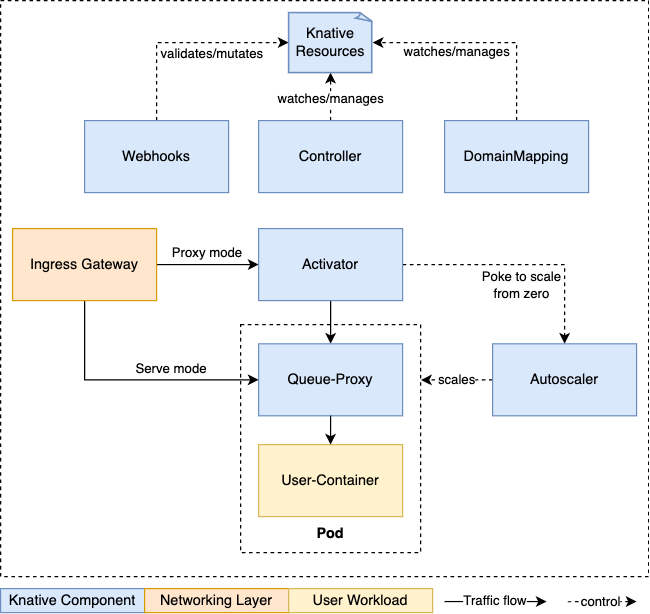
\includegraphics[width=.8\textwidth]{background/knative_serving_architecture.png}
    \caption[Knative Serving architecture components]{High-level architecture components of Knative Serving. Picture from \href{https://knative.dev/docs/serving/architecture/\#diagram}{Knative}.}
    \label{fig:knative_serving_architecture}
\end{figure}

\texttt{Activator} Is responsible for queueing incoming requests when a Knative Service is scaled to zero. It communicates directly with the autoscaler to reactivate services scaled to zero and forward queued requests. It can also act as a request buffer to handle traffic bursts.

\texttt{Autoscaler} Receives the request metrics and enables a suitable number of \gls{pod}s for the correct handling of this load.

\texttt{Controller} Watches the state of Knative resources within the cluster, manages the lifecycle of dependent resources, and updates the resource state.

\texttt{Queue-Proxy} Is a side-car \gls{container} in front of the user-container, collecting metrics and enforcing the desired concurrency when forwarding requests. When necessary, it can also act as a queue, similar to the \texttt{Activator}.

\texttt{Webhooks} They are responsible for the validation and mutation of Knative Resources.

A note must be made about the \texttt{Ingress} component. It does not refer to the \gls{k8s} Ingress Resource but to the concept of exposing external access to a resource on the cluster. This is possible thanks to the \texttt{Ingress} resource and the three layers of network abstraction available and supported by the community: Kourier, Contour and Istio.

\subsubsection{\acrfull*{KPA}}
The Knative Serving module provides an automatic scaling of revisions to meet incoming demand. By default, the \acrshort{KPA} is active and supports different metrics such as concurrency, requests-per-second, CPU and memory. In particular, the concurrency metric allows you to specify a soft constraint and a hard constraint, so you have more control over the number of running \gls{pod}s based on the use case.

The \acrfull{HPA} provided by \gls{k8s} is not part of the Knative Serving core. If you wish to use it, you must add it as an extension after installing Knative Serving.

\subsection{Eventing}
Knative Eventing is a collection of \acrshort{API}s that enables developers to easily follow an event-driven architecture with their applications. The Eventing module components allow events to be routed from producers (referred to as \texttt{Sources}) to consumers (referred to as \texttt{Sinks}) without worrying about the event format because it is consistent with the CloudEvents specification, a useful \acrshort{CNCF} project to standardize communication, which will be described below.

\begin{figure}[H]
    \centering
    \begin{subfigure}[t]{.9\textwidth}
        \centering
        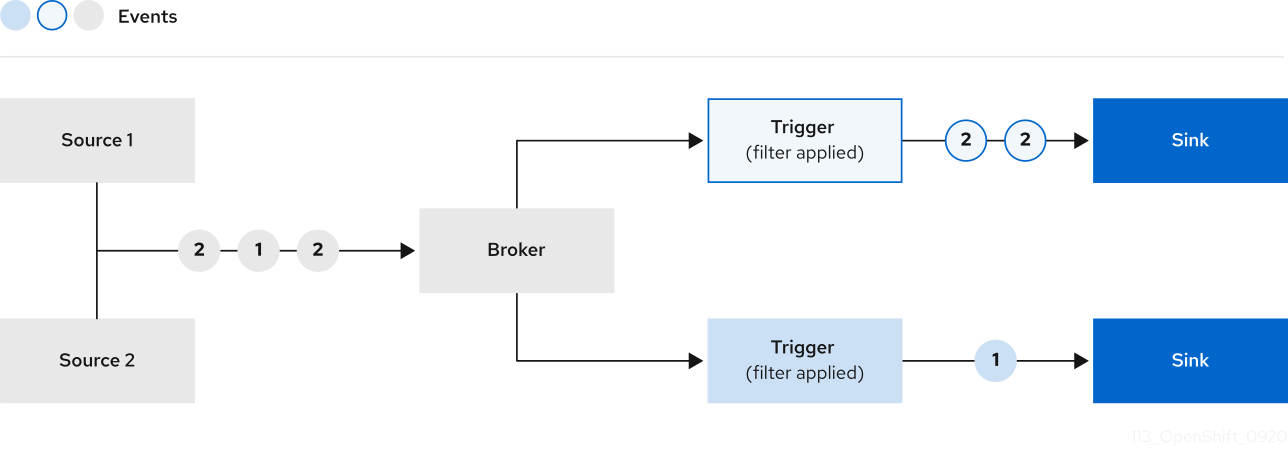
\includegraphics[width=\linewidth]{background/knative_eventing_architecture.png}
        \caption{Event producers send events to a \texttt{Broker} by POSTing the event, then the \texttt{Broker} uses \texttt{Triggers} for event delivery.}
        \label{fig:knative_eventing_broker}
    \end{subfigure}
    \vfill
    \begin{subfigure}[t]{.9\textwidth}
        \centering
        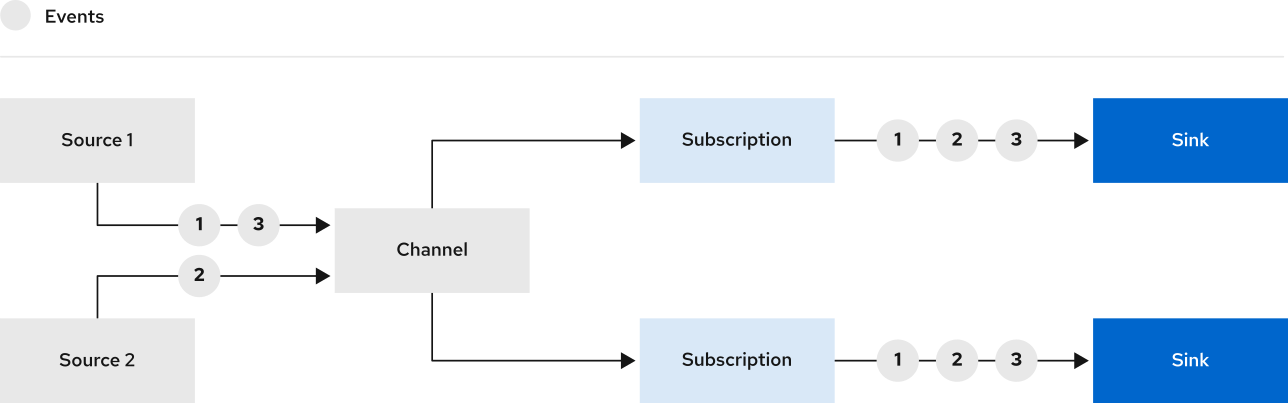
\includegraphics[width=\linewidth]{background/knative_eventing_channel.png}
        \caption{Event producers exploit \texttt{Channel} to fan out received events via \texttt{Subscriptions}.}
        \label{fig:knative_eventing_channel}
    \end{subfigure}
    \caption[Event-driven workflow examples]{Examples of event-driven workflow using different architectures and resources. Pictures from Knative \href{https://knative.dev/docs/eventing/brokers/}{(a)}\href{https://knative.dev/docs/eventing/channels/}{(b)}.}
    \label{fig:knative_eventing_architecture}
\end{figure}

Diagrams of possible applications using Knative Eventing can be seen in \autoref{fig:knative_eventing_architecture}. The main components are described below:

\texttt{Sources} Any \gls{k8s} object that generates or imports an event and transmits it to another endpoint on the cluster via CloudEvents. The resource that receives the event is an \texttt{Addressable} (e.g. \texttt{Sink}, \texttt{Broker}, etc.). Only a few of the various types available are listed:

\begin{itemize}
    \item \textit{APIServerSource}, produces a new event each time a \gls{k8s} resource is created, updated or deleted, bringing the \gls{k8s} \acrshort{API} into Knative;
    \item \textit{PinSource}, allows events production with fixed payload based on a specified Cron\footnote{Cron is a daemon software that runs continuously in the background and wakes up to handle periodic service requests when required. See \href{https://en.wikipedia.org/wiki/Cron}{https://en.wikipedia.org/wiki/Cron} for more details.} schedule;
    \item \textit{GitHub}, produces a new event for selected GitHub event types, bringing GitHub events into Knative;
    \item \textit{RabbitMQ}, brings RabbitMQ messages into Knative.
\end{itemize}

\texttt{Broker} Accumulates a pool of events defining an event mesh. It uses \texttt{Triggers} for event delivery and manages the delivery failures.

\texttt{Triggers} When an event is taken into account by the \texttt{Broker}, it can be forwarded to subscribers using this resource. They allow events to be filtered by attributes so that events with particular attributes can be sent to \texttt{Subscribers} that have registered interest in events with those attributes.

\texttt{Subscribers} Represents any \acrshort{URL} or \texttt{Addressable} resources. They can also reply to an active request from the \texttt{Broker} and can respond with a new event that is sent back to the \texttt{Broker}.

\texttt{Channel} Defines a single event forwarding and persistence layer. There are various types available:

\begin{itemize}
    \item \textit{InMemoryChannel}, the best effort was provided using an in-memory channel, not suitable for a production environment;
    \item \textit{KafkaChannel}, backed by Apache Kafka topics;
    \item \textit{NatssChannel}, backed by NATSS Streaming.
\end{itemize}

\texttt{Sinks} It is an \texttt{Addressable} or a \texttt{Callable} resource that can receive incoming events from other resources.

\begin{itemize}
    \item \texttt{Addressable} Receives and acknowledges an event delivered over \acrshort{HTTP} to an address defined in their \texttt{status.address.url} field. As a special case, the core \gls{k8s} Service object also fulfils the \texttt{Addressable} interface.
    \item \texttt{Callable} Receives an event sent via \acrshort{HTTP} and processes it, returning 0 or 1 new event in the \acrshort{HTTP} response. This returned event can be further processed in the same way as events from an external event source.
\end{itemize}

All these resources make it possible to achieve a mixed infrastructure, with different \texttt{Sources} producing events which are processed and forwarded, as shown in \autoref{fig:knative_eventing_mesh}.

\begin{figure}[H]
    \centering
    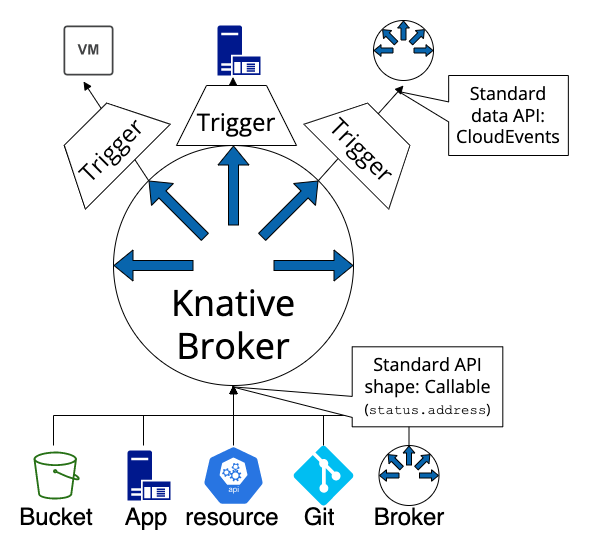
\includegraphics[width=.75\textwidth]{background/knative_eventing_mesh.png}
    \caption[Event mesh diagram]{Diagram showing event mesh mechanism, defined by \texttt{Broker} and \texttt{Triggers} \acrshort{API}s. Picture from \href{https://knative.dev/docs/eventing/event-mesh/}{Knative}.}
    \label{fig:knative_eventing_mesh}
\end{figure}

\subsubsection{CloudEvents}
Nowadays, there isn't a common way of describing events; developers have to write new event-handling logic for each event source. This lack of a common event format also results in the absence of uniform libraries, tools, and infrastructure for transmitting event data across different environments.

CloudEvents \cite{site:cloudevents} is a specification for describing event data in common formats in order to provide interoperability across services, platforms and systems and wants to fill this gap by offering \acrshort{SDK}s for various programming languages (e.g. Go, JavaScript, Java, C\#, Ruby, PHP, PowerShell, Rust, and Python). These libraries can be used to build event routes, tracing systems, and other related tools, thus addressing the challenges posed by the absence of a common event format.

The \autoref{code:cloudevents_example} shows a CloudEvent example, where \texttt{id}, \texttt{source}, \texttt{specversion} and \texttt{type} are required fields; meanwhile, the others are optional\footnote{See \href{https://github.com/cloudevents/spec/blob/v1.0.2/cloudevents/spec.md}{https://github.com/cloudevents/spec/blob/v1.0.2/cloudevents/spec.md} for more details.}.

\begin{lstlisting}[language=json, captionpos=b, caption={[CloudEvent example in JSON format]Example of a CloudEvent in JSON format, with all necessary fields and the payload, defined by the \texttt{data} object.}, label={code:cloudevents_example}]
{
    "specversion" : "1.0",
    "type" : "com.example.type",
    "source" : "/example/source",
    "id" : "82C32673-0C78",
    "time" : "2020-04-10T01:00:05+00:00",
    "datacontenttype" : "application/json",
    "data" : {
        "foo": "foo"
    }
}
\end{lstlisting}

\subsection{Function}
Knative Function offers a simple programming model for using functions on Knative, eliminating the need for in-depth knowledge of Knative, \gls{k8s}, \gls{container}s or \gls{dockerfile}s. Developers can easily create, build, and deploy stateless, event-driven functions as Knative Services by using the \texttt{func} \cite{site:knative_cli_tools} \acrshort{CLI}.

When a function is built or executed, it automatically generates a \gls{container} image in \acrfull{OCI} \cite{site:oci_image} format, which is stored in a container registry\footnote{A container registry is a repository or collection of repositories, used to store and access container images. See \href{https://www.redhat.com/en/topics/cloud-native-apps/what-is-a-container-registry}{https://www.redhat.com/en/topics/cloud-native-apps/what-is-a-container-registry} for more details.}. Subsequently, each time the code is updated and the function is executed or deployed, the \gls{container} image is updated to reflect the changes. It also simplifies the project creation by providing templates for different languages (e.g. Python, Go, Java, TypeScript, etc.) and invocation formats (\acrshort{HTTP} or CloudEvent).

The \autoref{code:knative_function} shows how to install the \texttt{func} plugin and how the creation, execution and deployment of a function example works.

\begin{lstlisting}[language=bash, captionpos=b, caption={[How to install and use func plugin]An example of how to install the \texttt{func} plugin and use it to create, build, push and deploy a simple function.}, label={code:knative_function}]
#!/bin/bash

# Install func plugin
brew tap knative-extensions/kn-plugins
brew install func

# Create hello function
func create --language go --template cloudevents hello
cd hello

# Build and push
func build --registry <registry> --push

# Deploy on the current context
func deploy
\end{lstlisting}

\section{Puppeteer}\label{sec:puppeteer}
Puppeteer is a Node library which provides a high-level \acrshort{API} to control headless Chrome or Chromium over the DevTools Protocol \cite{site:puppeteer, site:puppeteer_overview}, which enables instrumentation, inspection, debugging, and profiling in some Blink-based\footnote{Blink is a browser engine forked from the WebCore component of WebKit. See \href{https://www.chromium.org/blink/}{https://www.chromium.org/blink/} for more details.} browsers. The instrumentation is categorized into different domains (e.g., \acrshort{DOM}, Debugger, Network, etc.), each defining supported commands and generated events, both of which are serialized as fixed-structure \acrshort{JSON} objects.

The headless attribute specifies a way to run the Chrome browser in a headless environment, essentially without its graphical user interface. All the modern web platform features provided by Chromium and the Blink rendering engine are available by \acrshort{CLI} and are useful for different web automation tasks, while also reducing resource usage. In December 2023, Chrome's Headless mode was updated due to the old implementation that was separated from the Headfull one and shipped as part of the same Chrome binary \cite{site:puppeteer_headless_new}. It was challenging to keep both implementations up-to-date, each with its own bugs and features; for these reasons, as shown in \autoref{fig:puppeteer_headless_new}, Chrome developers unified Headless and Headfull browsers in one code-base only.

\begin{figure}[H]
    \centering
    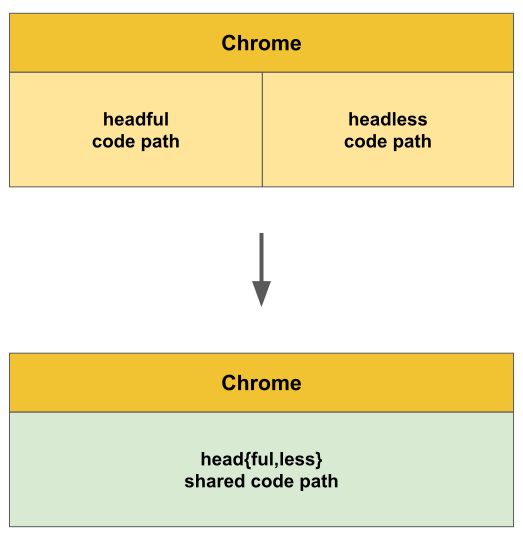
\includegraphics[width=.5\textwidth]{background/pptr_headless_new.png}
    \caption[Schema of the new Headless Chrome implementation]{Schema of the new Headless Chrome implementation. The old Headless Chrome was unified with the Headfull one. Picture from \href{https://developer.chrome.com/static/docs/chromium/new-headless/image/the-chrome-headless-is-7ec2038d11f0b.svg}{Chrome for developers}.}
    \label{fig:puppeteer_headless_new}
\end{figure}

Puppeteer was quickly updated to support this new Headless mode and in addition to the features it introduced, there are a lot of actions that can be performed using this library, for example:

\begin{itemize}
    \item generate screenshots and PDFs of pages;
    \item crawl a \acrlong{SPA} and generate pre-rendered content;
    \item automate actions such as form submission, UI testing and keyboard input;
    \item create an up-to-date, automated testing environment to directly run tests in the latest version of Chrome using the latest JavaScript and browser features;
    \item capture a timeline trace of your site to help diagnose performance issues;
    \item intercept and manipulate network requests;
    \item test Chrome extensions.
\end{itemize}

The Chrome Browser Automation team oversees maintenance, but being open-source actively encourages and welcomes community support and contributions. Users can choose which of the two available packages to install: \texttt{puppeteer} or \texttt{puppeteer-core}. The first includes, by default, the download of a recent version of Chrome for Testing\footnote{Chrome for Testing has been created purely for browser automation and testing purposes and is not suitable for daily browsing. See \href{https://developer.chrome.com/blog/chrome-for-testing/}{https://developer.chrome.com/blog/chrome-for-testing/} for more details.} while the latter doesn't. 

\autoref{fig:puppeteer_overview} shows an overview of the library architecture with all the basic components that make the operations described above possible.

\begin{figure}[H]
    \centering
    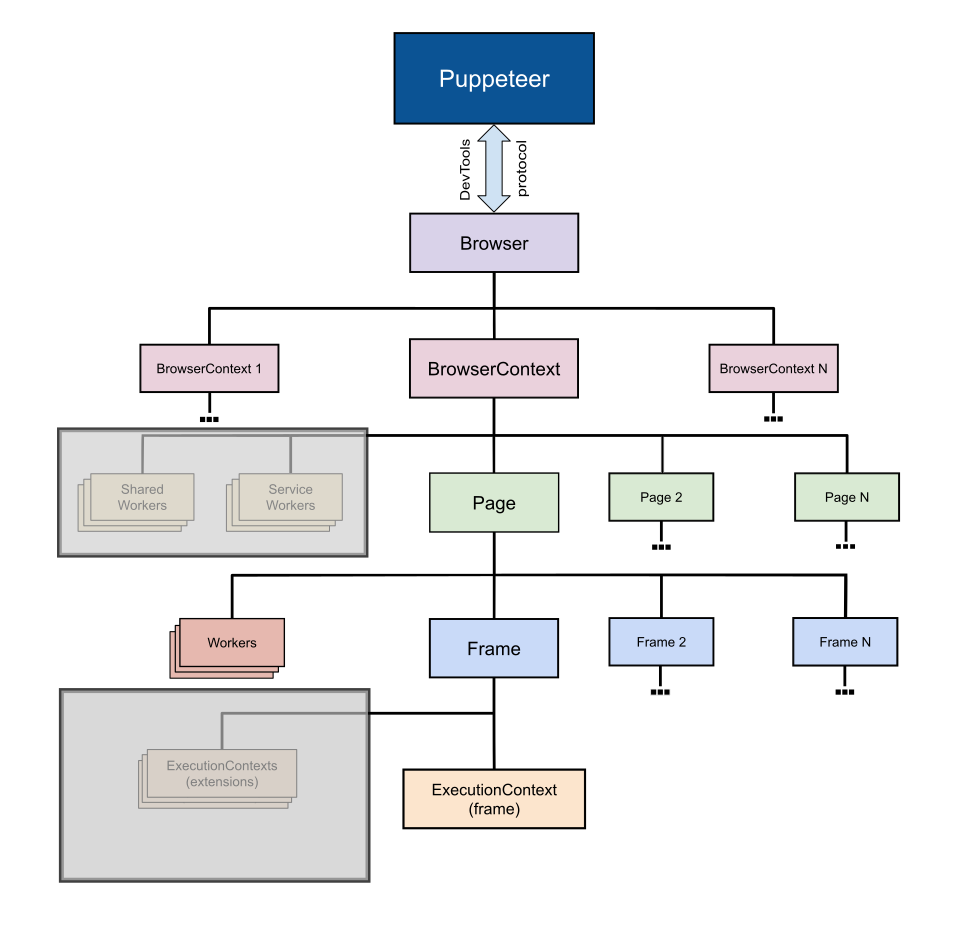
\includegraphics[width=.8\textwidth]{background/pptr_overview.png}
    \caption[Puppeteer architecture overview]{Overview of the Puppeteer library architecture. Picture from \href{https://raw.githubusercontent.com/puppeteer/puppeteer/main/docs/assets/overview.png}{GitHub}.}
    \label{fig:puppeteer_overview}
\end{figure}

\subsection{Stealth plugin}
Although Puppeteer is a robust library, it has limitations regarding extensibility and customization. For these reasons, a German developer named berstend on GitHub created a modular plugin framework built on top of Puppeteer called Puppeteer-Extra \cite{site:puppeteer_extra_wiki}.

One of the most widely used is \texttt{puppeteer-extra-plugin-stealth} \cite{site:puppeteer_extra_stealth}, which deals with applying various evasion techniques to make the detection of puppeteers harder. It's probably impossible to prevent all ways to detect Headless Chromium, but it should be possible to make it so complicated that it becomes cost-prohibitive or triggers too many false positives to be feasible. Other relevant plugins are:

\begin{itemize}
    \item \texttt{puppeteer-extra-plugin-recaptcha}, solves reCAPTCHAs\footnote{reCAPTCHA is a free service from Google that helps protect websites from spam and abuse. See \href{https://www.google.com/recaptcha/about/}{https://www.google.com/recaptcha/about/} for more details.} automatically, using a single line of code;
    \item \texttt{puppeteer-extra-plugin-adblocker}, very fast and efficient blocker for ads and trackers that reduces bandwidth and load times;
    \item \texttt{puppeteer-extra-plugin-anonymize-ua}, anonymizes the user-agent on all pages using dynamic replacing, so the browser version stays intact and recent.
\end{itemize}

\section{Elasticsearch}\label{sec:elasticsearch}
Elasticsearch is a distributed search and analysis engine at the heart of Elastic Stack. Together with Kibana, Beats and Logstash, they form the ELK Stack: a product that allows reliable and secure data to be taken from any source and any format, with the aim of searching, analyzing and visualizing it.

\begin{figure}[H]
    \centering
    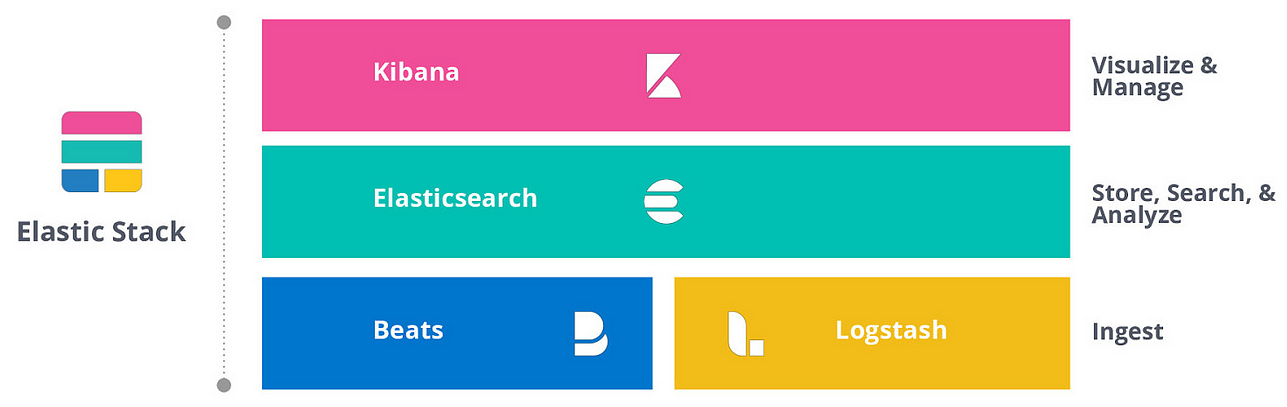
\includegraphics[width=1\textwidth] {background/elastic_stack_overview.png}
    \caption[\acrshort{ELK} Stack overview]{Overview of the Elastic Stack and its components. Picture from \href{https://miro.medium.com/v2/1*BR2dtNq9wkvZZdg4L4GbwQ.png}{Medium}.}
    \label{fig:elastic_stack_overview}
\end{figure}

As briefly illustrated in \autoref{fig:elastic_stack_overview}, each module has its own purpose and can be used separately. In particular, the Elasticsearch tool is built on top of Apache Lucene, a historical library with the same objective. It was developed due to the complexity of Lucene and it hides the hard Java integration behind a simple and coherent \acrshort{REST}ful \acrshort{API} \cite{book:elasticsearch_guide_2015}.

Since its first release, it has been distributed with open-source Apache License 2.0. However, in January 2021, with the release of Elasticsearch 7.11, the Elastic company decided to change the licence of Elasticsearch and Kibana to a dual, not open-source license: Elastic License and \acrfull{SSPL}. This choice was made to prevent Amazon, and other companies, from providing Elasticsearch and Kibana as a service without collaborating with Elastic \cite{site:elasticsearch_license, site:elasticsearch_vs_amazon}.

To understand the functionality of Elasticsearch better and to discover its benefits, it is useful to describe what an index is. The index concept in Elasticsearch can be compared to an optimized collection of documents, each document is a compilation of fields represented as key-value pairs. By default, Elasticsearch indexes all data in each field and each indexed field has a dedicated and optimized data structure (e.g. text fields are stored in inverted indices, numeric and geoinformation fields are stored in BKD trees, etc.). This approach enables the efficient and specialized handling of different types of data, contributing to the platform's effectiveness in managing and retrieving various forms of information in near real-time \cite{site:elasticsearch_doc_index}. When the document is actually stored, searches can be directly performed using the \acrshort{REST} \acrshort{API} or the Elasticsearch client available in different programming languages; both support structured queries, full-text queries and complex queries combining the two.

In addition to the index concept, it is essential to understand the fundamental components that make up the Elasticsearch backend. These components are depicted in \autoref{fig:elasticsearch_be_components} and include:

\begin{itemize}
    \item a cluster, defined as a group of one or more node instances that are connected together;
    \item one or more nodes, each representing a single server that stores data and participates in the cluster's indexing and search capabilities;
    \item shards, each representing a subset of the data stored in an index, are extremely useful for distributing the workload across multiple nodes;
    \item documents, as described above, are the basic unit of information and consist of a \acrshort{JSON} object with key-value pairs that represent the data to be stored and indexed.
\end{itemize}

\begin{figure}[H]
    \centering
    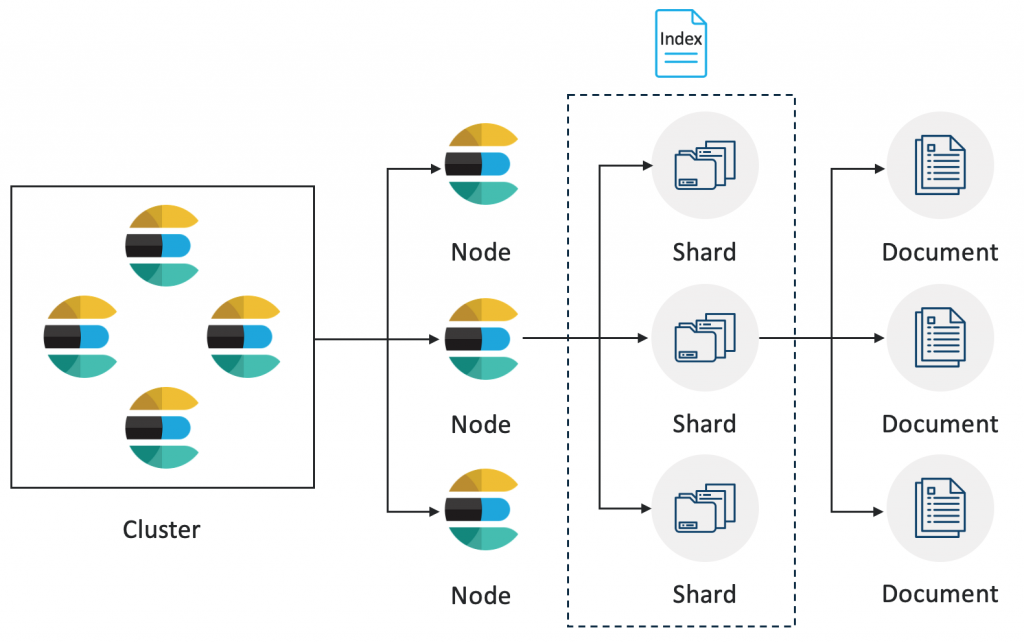
\includegraphics[width=.8\textwidth]{background/elasticsearch_be_components.png}
    \caption[Elasticsearch backend components]{Architecture of an Elasticsearch installation, with all key components. Picture from \href{https://blog.miraclesoft.com/wp-content/uploads/2023/08/xelasticsearch-image-1-1024x643.png.pagespeed.ic.DhHOg8eTFd.webp}{Miracle}.}
    \label{fig:elasticsearch_be_components}
\end{figure}

It is important to specify that there are different types of nodes, such as master nodes, data nodes, ingest nodes and others, each with a specific role in the cluster. Furthermore, it is necessary to have at least one master node and three master-eligible nodes to keep the cluster healthy and enable the platform to operate properly, even in the event of failures.

\subsection{Elastic Cloud on Kubernetes}
There are different ways to install Elasticsearch. You can use the hosted service, manually install it, use package managers, run it on \gls{container}s with \gls{docker}, deploy it with Helm charts, or use \acrfull{ECK}. The latter, in our scenario, is the most interesting way.

In May 2019, Elastic announced this new orchestration product based on the \gls{k8s} Operator pattern\footnote{Operators are software extensions to \gls{k8s} that make use of custom resources to manage applications and their components following \gls{k8s} principles. See \href{https://kubernetes.io/docs/concepts/extend-kubernetes/operator/}{https://kubernetes.io/docs/concepts/extend-kubernetes/operator/} for more details.} that allows users to make available, manage and operate Elasticsearch clusters on \gls{k8s} \cite{site:elasticsearch_kubernetes}. It was called \acrshort{ECK} and focuses not only on simplifying the task of deploying Elasticsearch and Kibana but also on streamlining critical operations such as managing and monitoring multiple clusters, upgrading to new stack versions, scaling cluster capacity, changing cluster configuration, dynamically scaling local storage, and scheduling backups.

A step-by-step guide for installing the \acrshort{ECK} operator and deploying an Elasticsearch cluster is given in \autoref{code:eck_yaml_installation} and \ref{code:elasticsearch_quickstart}.

\begin{lstlisting}[language=bash, captionpos=b, caption={[How to install ECK operator]Install ECK operator with its \acrshort{CRD}s and RBAC rules.}, label={code:eck_yaml_installation}]
#!/bin/bash
ECK="https://download.elastic.co/downloads/eck/2.11.0"

# Install custom resource definitions (CRDs)
kubectl create -f "${ECK}/crds.yaml"

# Install the operator with RBAC rules
kubectl apply -f "${ECK}/operator.yaml"
\end{lstlisting}

\begin{lstlisting}[language=yaml, captionpos=b, caption={[Elasticsearch quickstart deploy]Elasticsearch cluster specification to deploy one Elasticsearch node.}, label={code:elasticsearch_quickstart}]
apiVersion: elasticsearch.k8s.elastic.co/v1
kind: Elasticsearch
metadata:
  name: quickstart
spec:
  version: 8.12.0
  nodeSets:
  - name: default
    count: 1
    config:
      node.store.allow_mmap: false
\end{lstlisting}

\end{document}